\chapter{Numerical experiments}
\label{chap:expe}

From the point of view of computational cost, it is convenient to make a brief analysis of the relevant new continuous-time framework obtained in Eq. \ref{eqn:u3.3}. The main problem that we can find when dealing with large networks (matrices) resides in the computation of the matrix logarithm, which can be computationally expensive.

This function computes the natural logarithm of a matrix, which is defined as follows \cite{higham2008functions}:

\begin{definition}
    A logarithm of $A \in \mathbb{C}^{N\times N}$ is any matrix $X$ such that $e^X = A$ where $e^X = I + X + \frac{X^2}{2!} + \frac{X^3}{3!} + \cdots$. If $A$ is assumed to have no eigenvalues on $\mathbb{R}^{-}$, then we call this logarithm to be the principal logarithm of $A$, which is the unique logarithm whose spectrum lies in the strip $\{ z : −\pi < Im(z) < \pi \}$.
\end{definition}

The matrix logarithm can be approximated by its Taylor series expansion. The Taylor series expansion of the matrix logarithm of a matrix $I - \alpha A$ can be expressed as:

$$log(I - \alpha A) = \sum_{k=1}^{\infty} (-1)^{k+1}\frac{\alpha^k}{k}A^k$$

where $I$ is the identity matrix of size $N$.

The accuracy of the approximation depends on the value of $k$, which determines how many terms in the series are included. The higher the value of $k$, the more accurate the approximation, but also the more computationally expensive it is to compute.

It's worth noting that for certain matrices, the Taylor series expansion may not converge or may converge too slowly to be practical for approximating the matrix logarithm. In such cases, other approximation methods like the Padé approximation or Schur decomposition may be more effective \cite{higham2008functions}.

In Python, the \texttt{scipy.linalg.logm} module from the SciPy library computes the logarithm of a matrix using the Schur decomposition with a computational cost of $\mathcal{O}(N^3)$ for an $N \times N$ matrix. However, the Schur decomposition is not always the most efficient way to compute the matrix logarithm, especially for large matrices with special properties such as sparsity or symmetry. In these cases, specialized algorithms, based on Krylov methods, rational approximations or iterative methods plus preconditioning, may be used to approximate the matrix logarithm to reduce its computational cost.

Next, we consider the two synthetic experiments from \cite{grindrod2014dynamical} in order to demonstrate how our new matrix ODE approach works and provide a better understanding of the $\alpha,\beta$ parameters. With this two artificial networks that evolve continuously over time, we intend to show a hierarchy of influence for the nodes that would not be evident if we only considered a static picture or a summarized view of the network. The relatively small size of these examples, 31 and 17 nodes respectively, will facilitate the process of visualizing, and it will also allow us to employ a highly precise Runge-Kutta iteration to solve the corresponding ODE systems (\ref{eqn:u3.3}) with accuracy.

\section{Synthetic experiments}
\label{sec:synexp}
The first synthetic experiment models a cascade of information through the directed binary
tree structure illustrated in Figure \ref{fig:exp1}. On a time interval $t = [0, 20]$, the adjacency
matrix $\mathbf{A}(t)$ of such network switches between two constant values $\mathbf{A}_{even}$ and $\mathbf{A}_{odd}$ on each sub-interval $[i, i + 1)$ for $i=0,1,2,\dots$, specifically

\begin{equation*}
\mathbf{A}(t)=
    \begin{cases}
        \mathbf{A}_{even}, & \text{if } mod(\lfloor t \rfloor, 2) = 0\\
        \mathbf{A}_{odd}, & \text{otherwise} 
    \end{cases}
\end{equation*}

where $\mathbf{A}_{even}$ is the adjacency matrix relative to the subgraph with solid edges in Figure \ref{fig:exp1}, and $\mathbf{A}_{odd}$ the one relative to the subgraph with dashed edges. Some noise to this structure is added by including extra directed edges that are chosen uniformly at random for each subinterval, with an average of five edges added each time. 

This type of structure allows us to clearly visualize the follow-on effect arising from the time-ordering of the node interactions.

\begin{figure}[h]\centering
    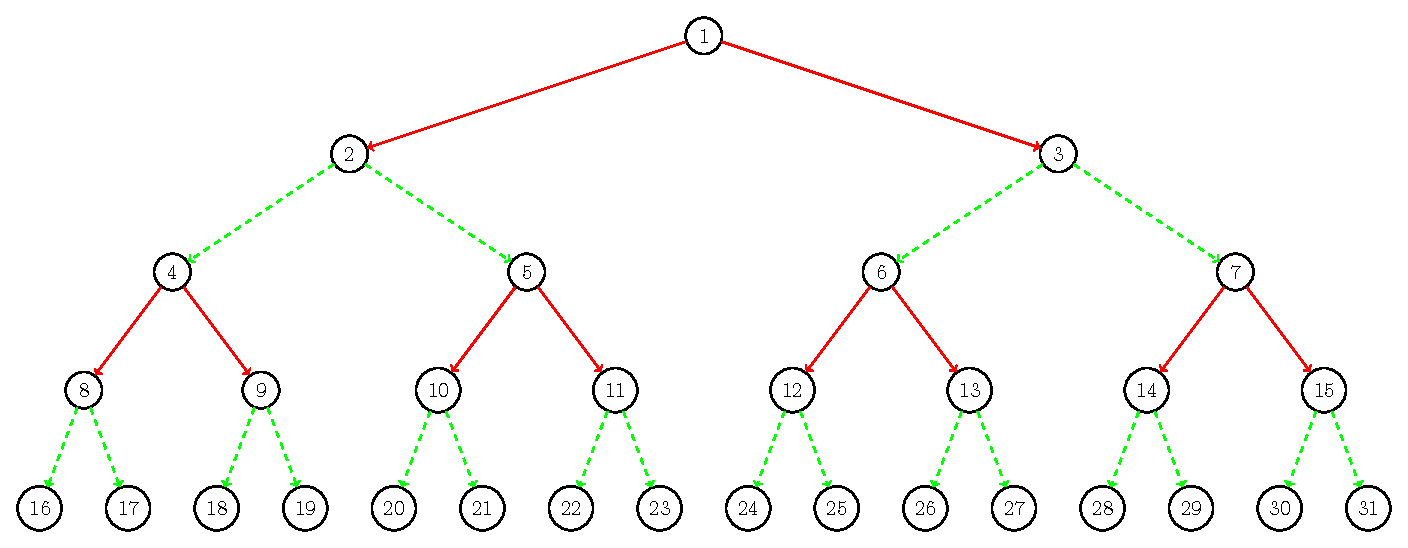
\includegraphics[width=.75\textwidth]{experiment1}
    \caption{Network structure (binary tree) for the first synthetic experiment. The active links of A(t) alternate between the solid and dashed edges, with extra noise added at each time step, over a period of 10 cycles.}
    \label{fig:exp1}
    \bigskip
\end{figure}

Due to the hierarchy and timing of the edges, information appears to flow from lower indices to higher. The binary structure of the tree makes node 1 to be particularly efficient at transmitting information through the network, although this may not be immediately apparent in a single snapshot.

Figure \ref{fig:bt1} displays the dynamic broadcast centrality from Eq. \ref{eqn:u3.4}, at time $t=20$ for each of the 31 nodes. We observe that node 1 has a strong advantage in terms of centrality, and that centrality tends to decrease as the index increases. Nodes 2 and 5 are ranked higher than node 3, indicating that the additional noise has affected this part of the network. Since the maximum spectral radius of $\mathbf{A}(t)$ over the interval $[0, 20]$ is one, the parameter $\alpha=0.7$ was chosen with $\beta=0.1$, in this case.

Figure \ref{fig:bt2} depicts the same results with a lower $\beta=0.01$ value, which increases the contribution of older walks. As a reminder, if we consider a walk starting at time zero, then the  downweighting factor becomes $e^{−20 \times 0.01} \approx 0.8$ rather than $e^{−20 \times 0.1} \approx 0.1$. This change of the $\beta$ parameter has a negligible effect on the node rankings which makes sense considering that the network dynamics have an underlying periodic pattern, but it can be observed that it generates larger absolute values.

In Figure \ref{fig:bt3}, we return to the original $\beta=0.1$ value and set $\alpha$ to 0.1, resulting in less marked differences in the node rankings. Even though node 1 continues to be the most central, the differences are less pronounced as its capability to initiate numerous dynamic walks of length 4 to nodes at the bottom of the hierarchy has less influence or weight.

Figure \ref{fig:bt4} illustrates the aggregate degree of each node, that is, the sum of out degrees over time for each node. For nodes 1 to 15 in the binary tree structure, this value is 20, which fluctuates due to the introduced noise. This graph highlights that the overall bandwidth can be a misleading network metric for determining node influence.

\begin{figure}[h]
     \centering
     \begin{subfigure}[b]{0.4\textwidth}
         \centering
         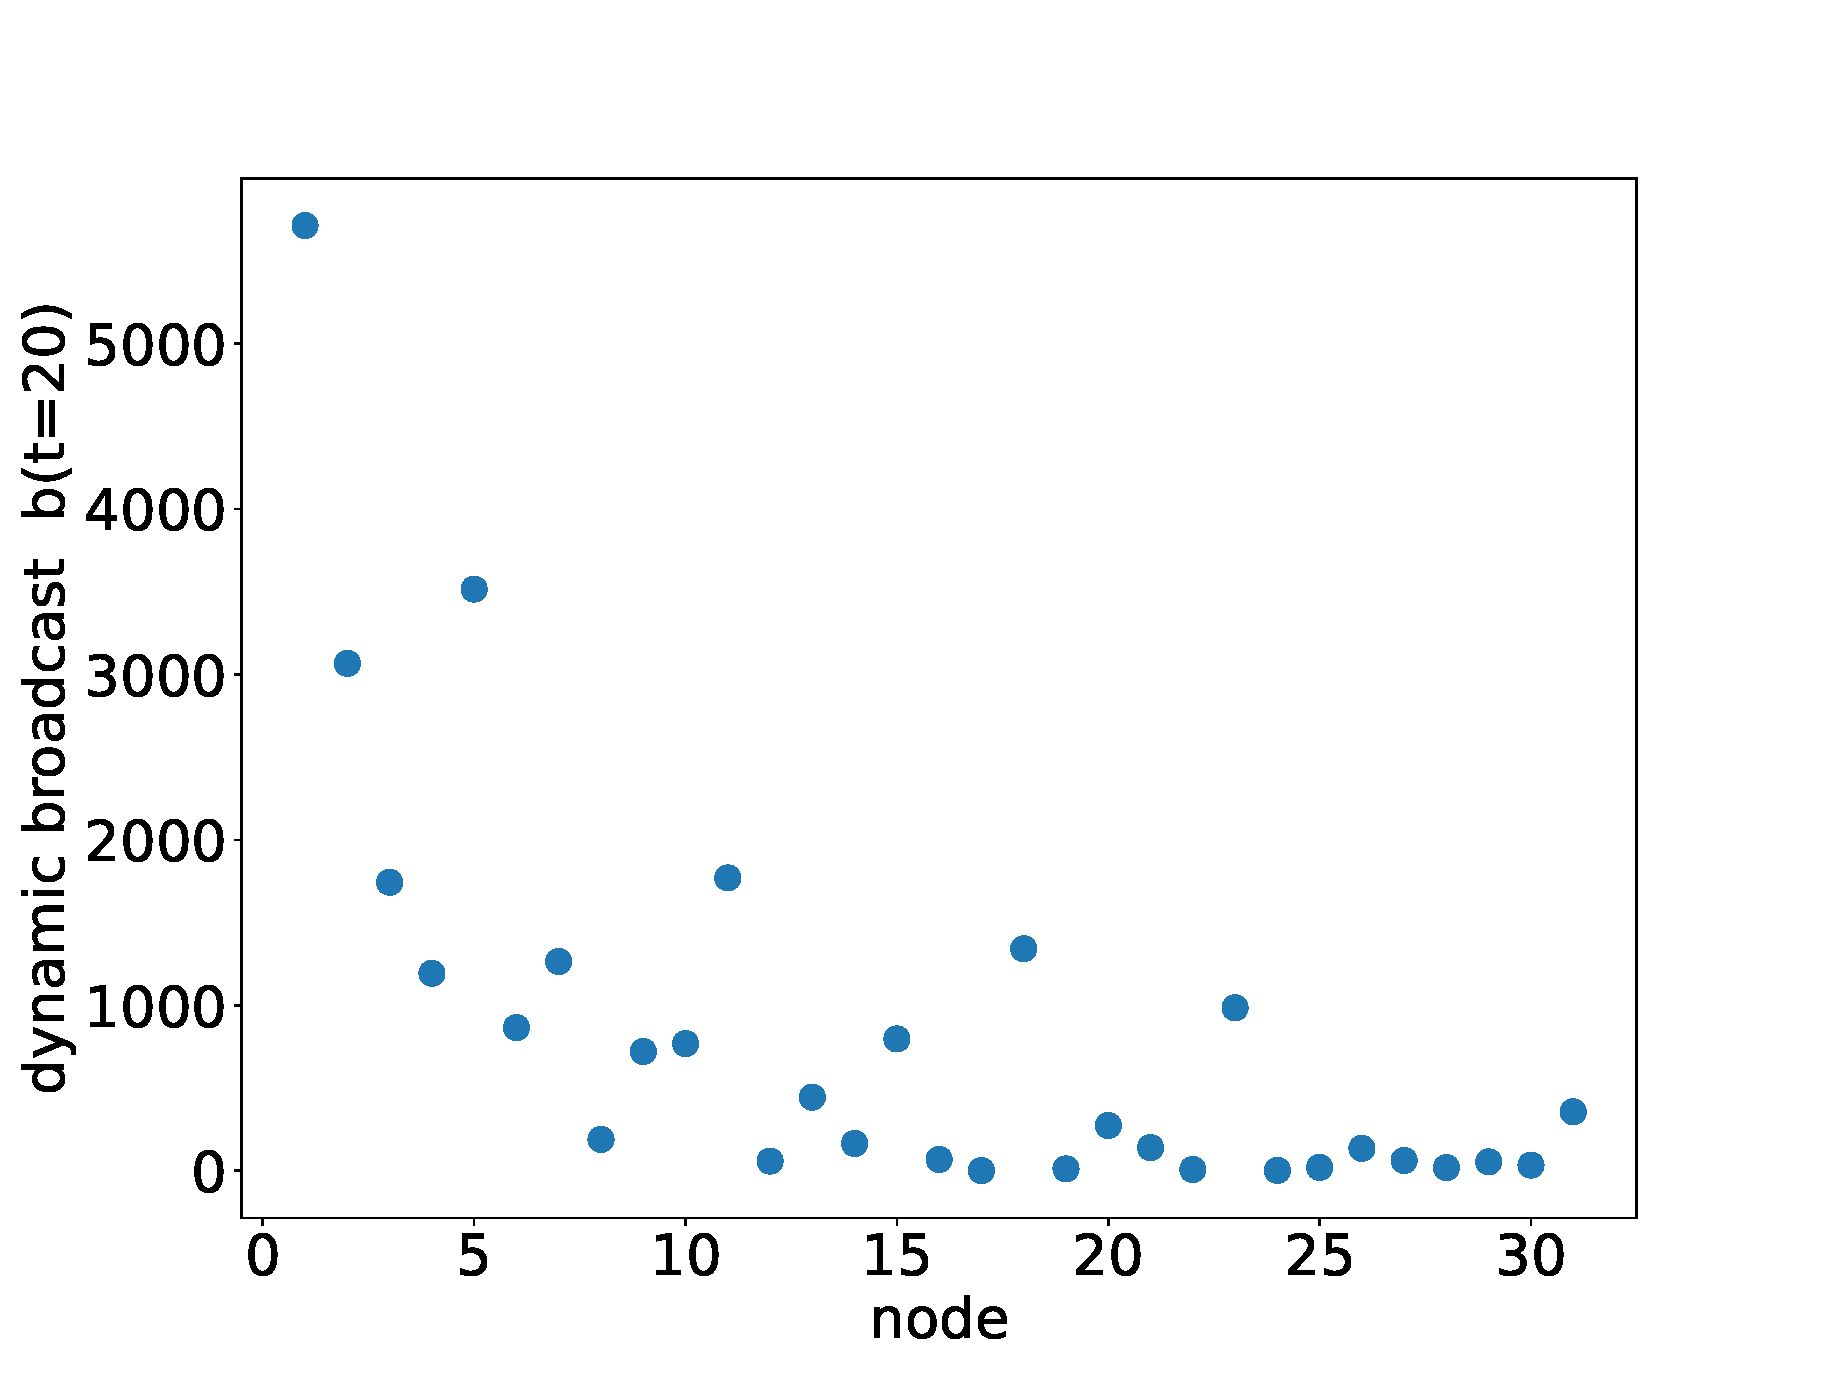
\includegraphics[width=\textwidth]{exp1_bt20a}
         \caption{Broadcast centrality for $\alpha = 0.7 ,~\beta = 0.1$}
         \label{fig:bt1}
     \end{subfigure}
     \hspace{0.5cm}
     \begin{subfigure}[b]{0.4\textwidth}
         \centering
         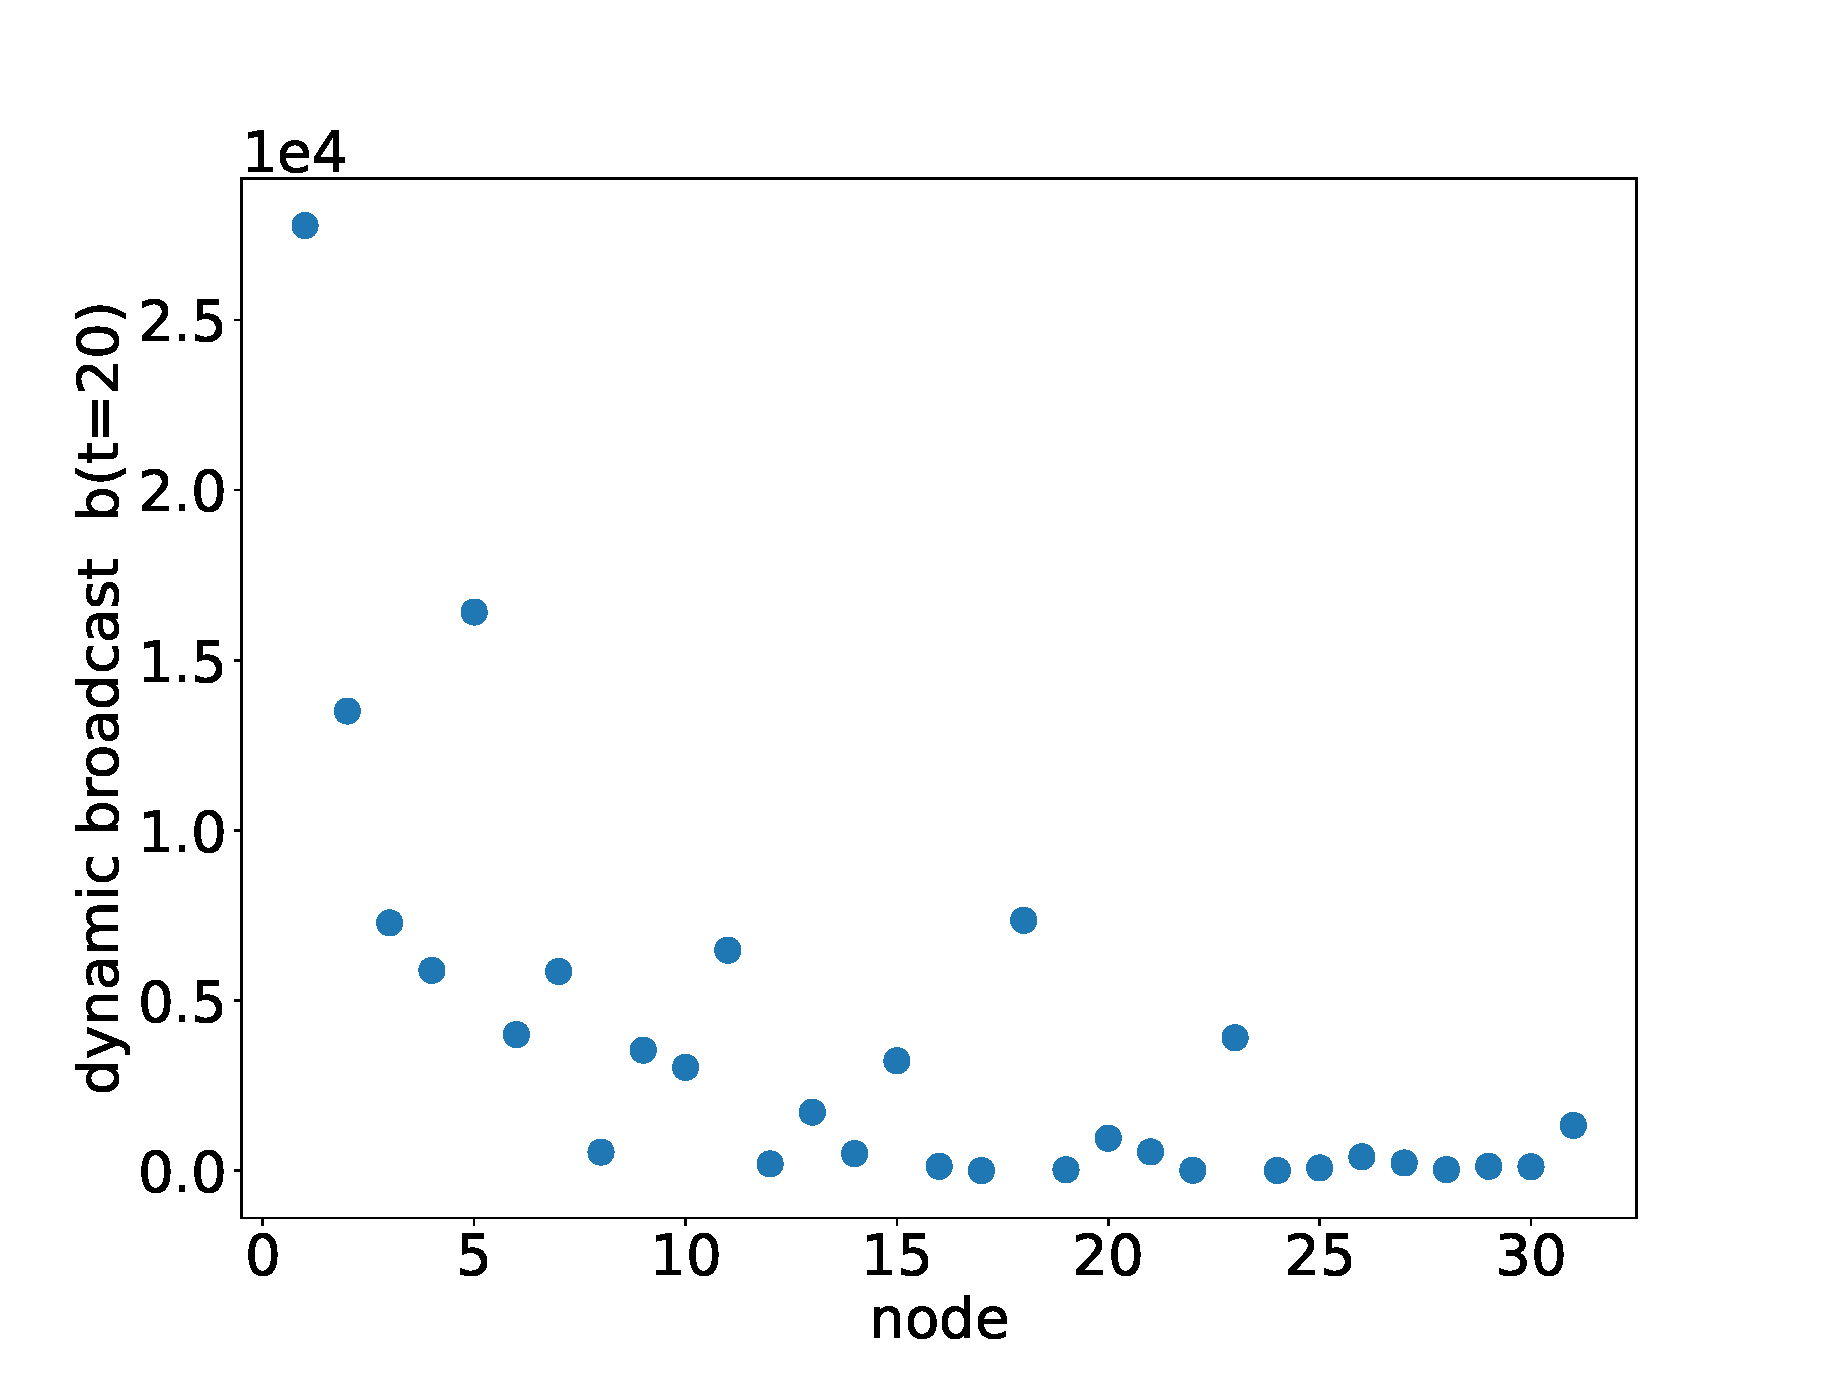
\includegraphics[width=\textwidth]{exp1_bt20b}
         \caption{Broadcast centrality for $\alpha = 0.7 ,~\beta = 0.01$}
         \label{fig:bt2}
     \end{subfigure}
     
     \begin{subfigure}[b]{0.4\textwidth}
         \centering
         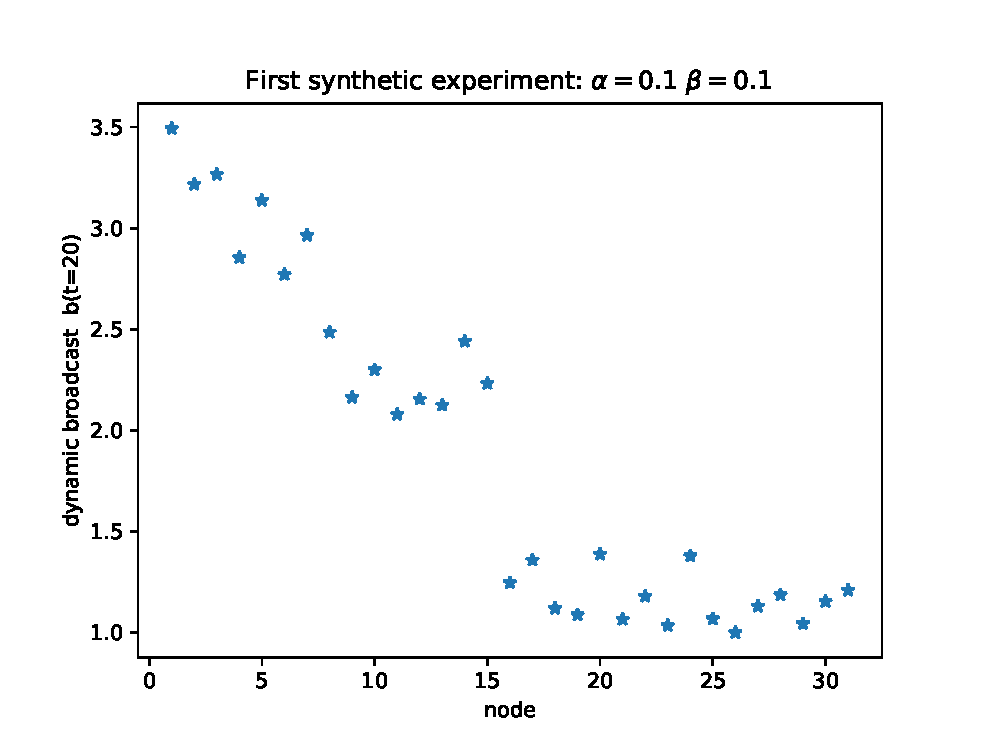
\includegraphics[width=\textwidth]{exp1_bt20c}
         \caption{Broadcast centrality for $\alpha = 0.1 ,~\beta = 0.1$}
         \label{fig:bt3}
     \end{subfigure}
     \hspace{0.5cm}
     \begin{subfigure}[b]{0.4\textwidth}
         \centering
         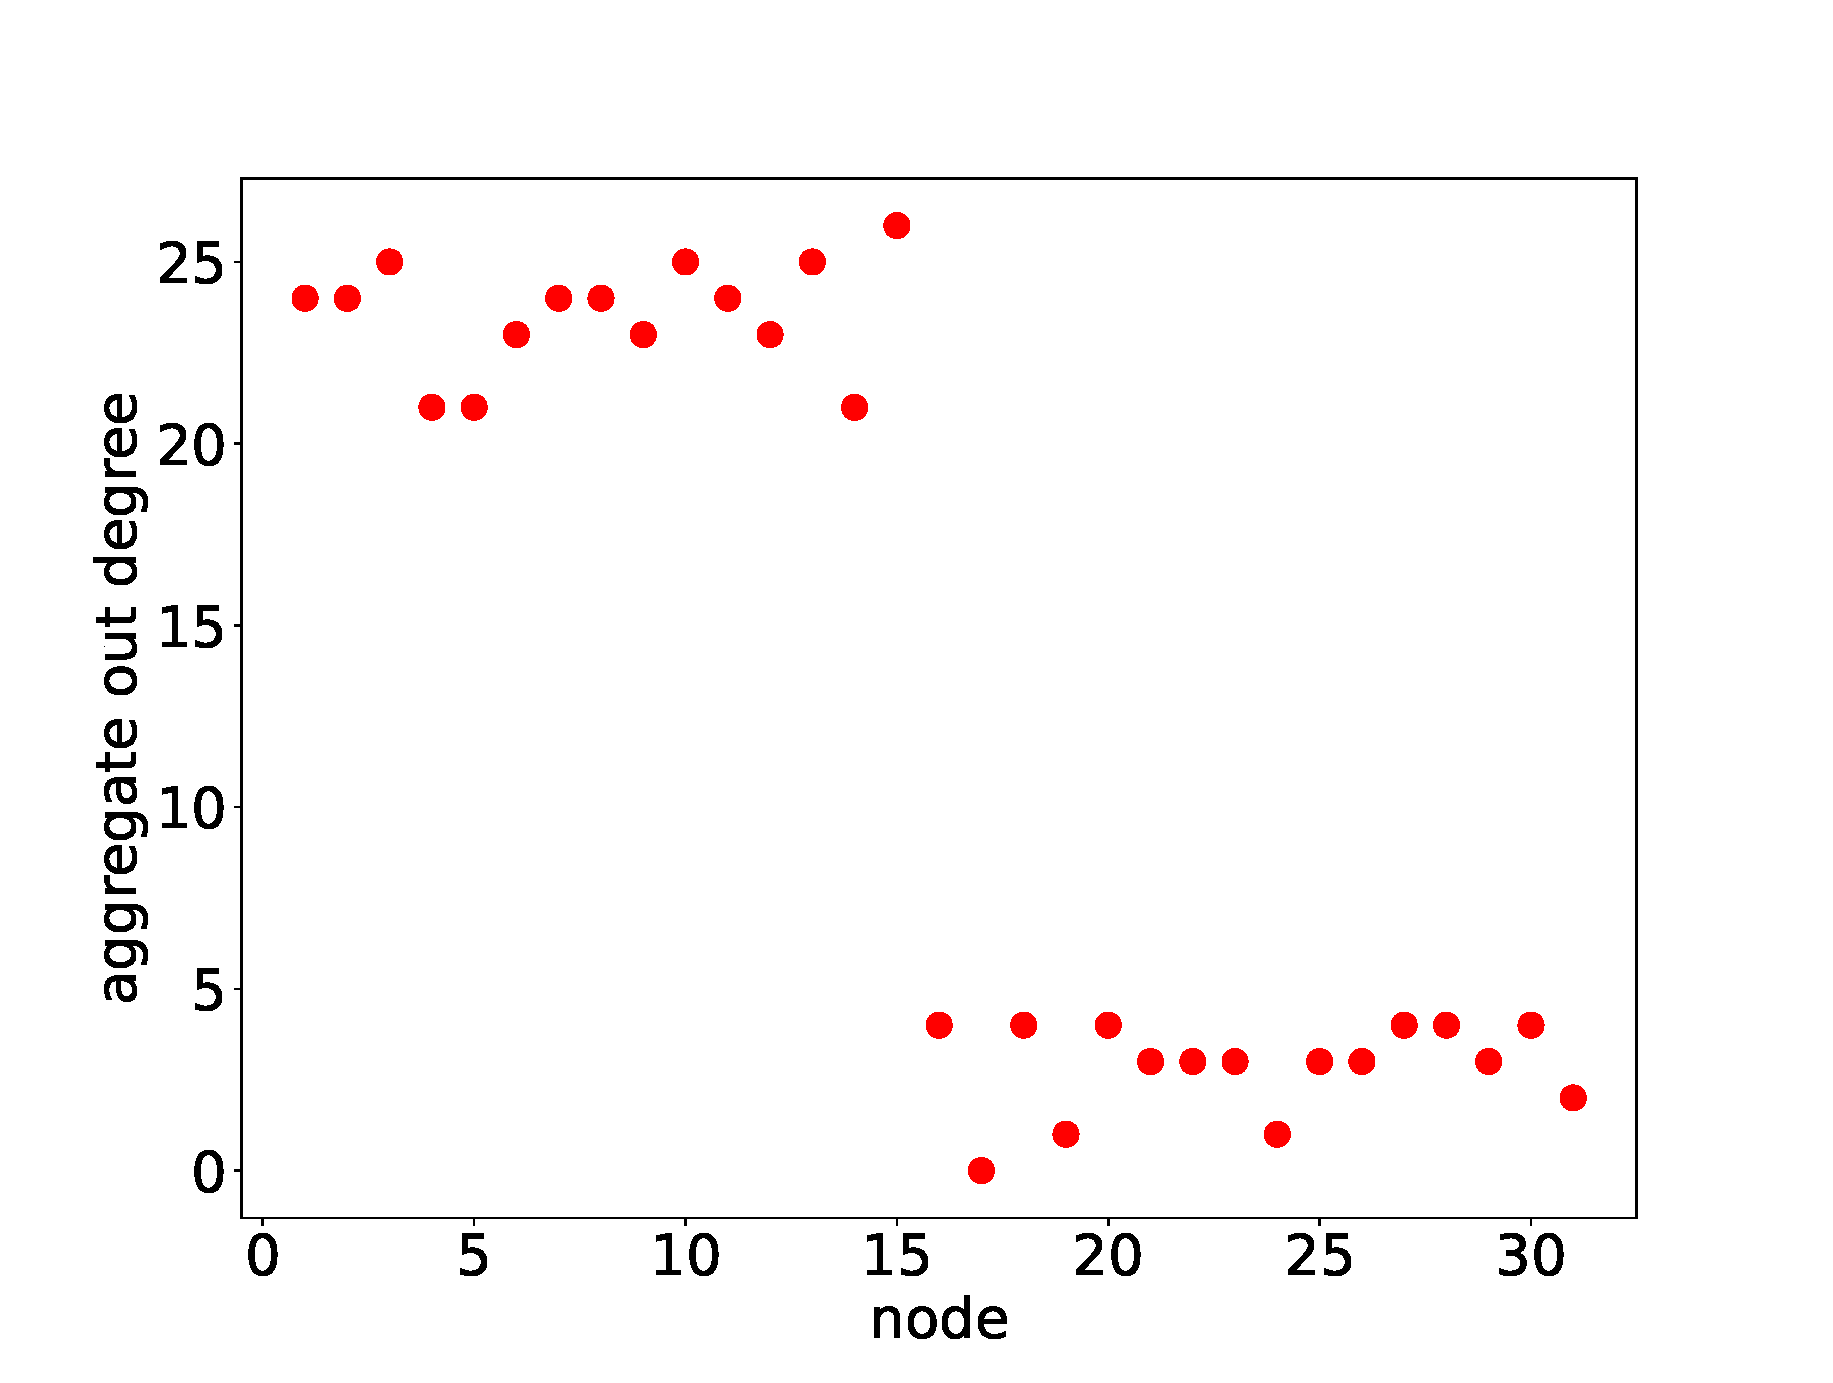
\includegraphics[width=\textwidth]{exp1_agg_out_degree}
         \caption{Aggregate out degree for each node}
         \label{fig:bt4}
     \end{subfigure}
        \caption{Results from the dynamic network in figure \ref{fig:exp1}.}
        \label{fig:fourbt}
\end{figure}

\newpage
We now consider the second synthetic experiment from \cite{grindrod2014dynamical}. The experiment simulates multiple rounds of voice calls that occur along an undirected binary tree structure. Each node in the tree has at most one active edge at any given time, meaning that there are no "conference" calls.  Figure \ref{fig:exp2} shows the network with labels assigned to the edges indicating when they are active. 

The adjacency matrix, $\mathbf{A}(t)$, for this experiment is defined based on the ordered and non-overlapping time intervals such that $t_i\coloneqq[(i − 1)\tau , (i − 1 + 0.9)\tau )$, for $i=0, 1, \dots , 7$, and $\tau =0.1$.

\begin{figure}[h]\centering
    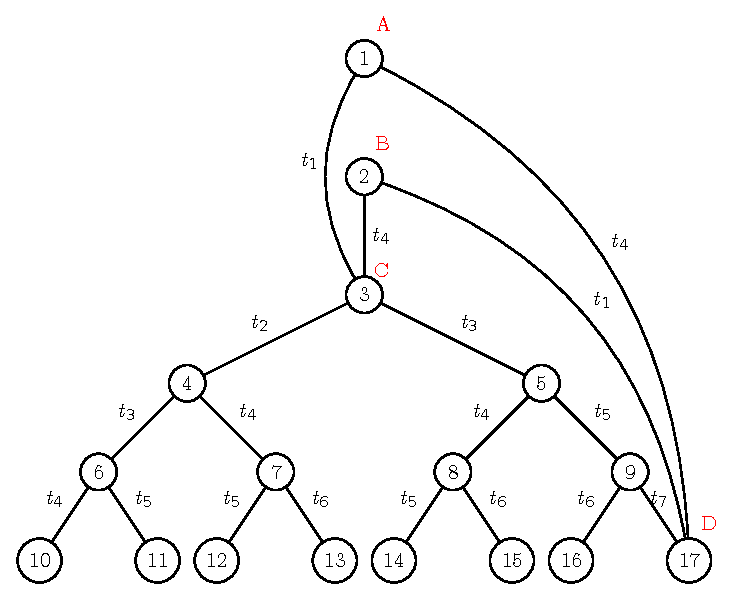
\includegraphics[width=.65\textwidth]{experiment2}
    \caption{Network structure for the second synthetic experiment. Links of A(t) are active over non-overlapping time intervals such that $t_i\coloneqq[(i − 1)\tau , (i − 1 + 0.9)\tau )$, for $i=0, 1, \dots , 7$, and $\tau =0.1$, repeated periodically over five cycles.}
    \label{fig:exp2}
    \bigskip
\end{figure}

The dynamic network is constructed in a way that node A is designed to be a more effective influencer compared to node B. This can be attributed to several factors such as a higher social/business status or access to more current and relevant information. Connections are built in such a way that node A talks to node C in $t_1$, initiating the cascade of phone calls in the network. On the other hand, node B waits until $t_4$ to contact node C, which does not trigger any new cascades. In this scenario, all the adjacency matrices for each time interval turn out to have unitary spectral radius.

The experiment is repeated over five cycles, during which nodes A and B send out a total of 10 messages. Even if nodes A and B have an apparent identical behaviour from an overall perspective, both contacting nodes C and D for the same length of time, the results in Figure \ref{fig:twobt} (for $\alpha = 0.7, \beta = 0.1$ and $\alpha = 0.9 , \beta = 0.1$ respectively) show that the dynamic broadcast centrality measure is able to capture the knock-on effect enjoyed by node A (solid line) with respect to node B (dashed line). This difference in broadcast centrality is much more pronounced for values of $\alpha$ close to one (Figure \ref{fig:bt6}), where longer walks are more strongly penalized.

\begin{figure}
     \centering
     \begin{subfigure}[b]{0.49\textwidth}
         \centering
         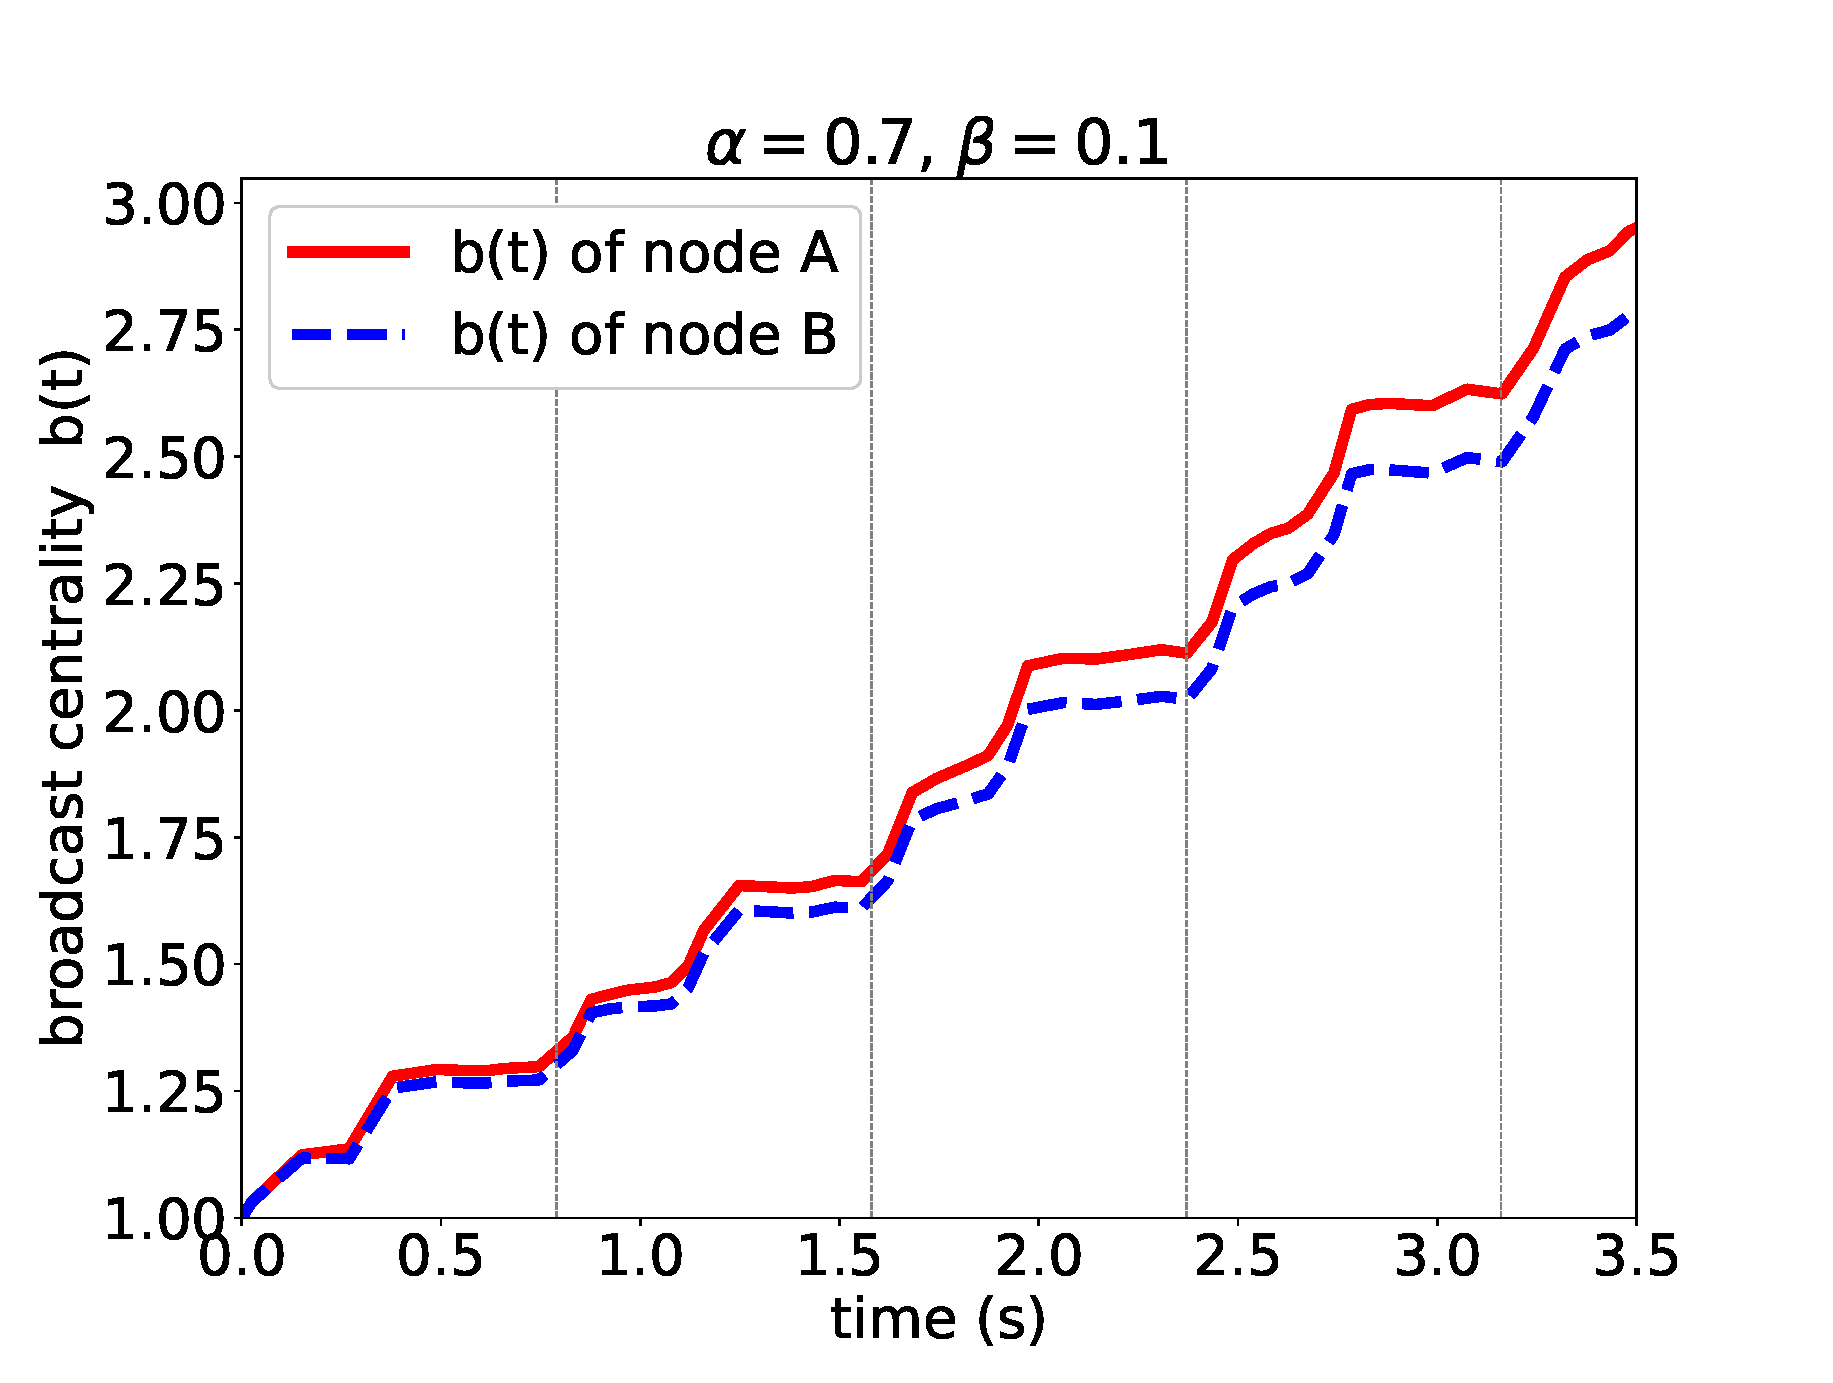
\includegraphics[width=\textwidth]{exp2b_btA_vs_btB}
         \caption{broadcast for $\alpha = 0.7 ,~\beta = 0.1$}
         \label{fig:bt5}
     \end{subfigure}
     \hfill
     \begin{subfigure}[b]{0.49\textwidth}
         \centering
         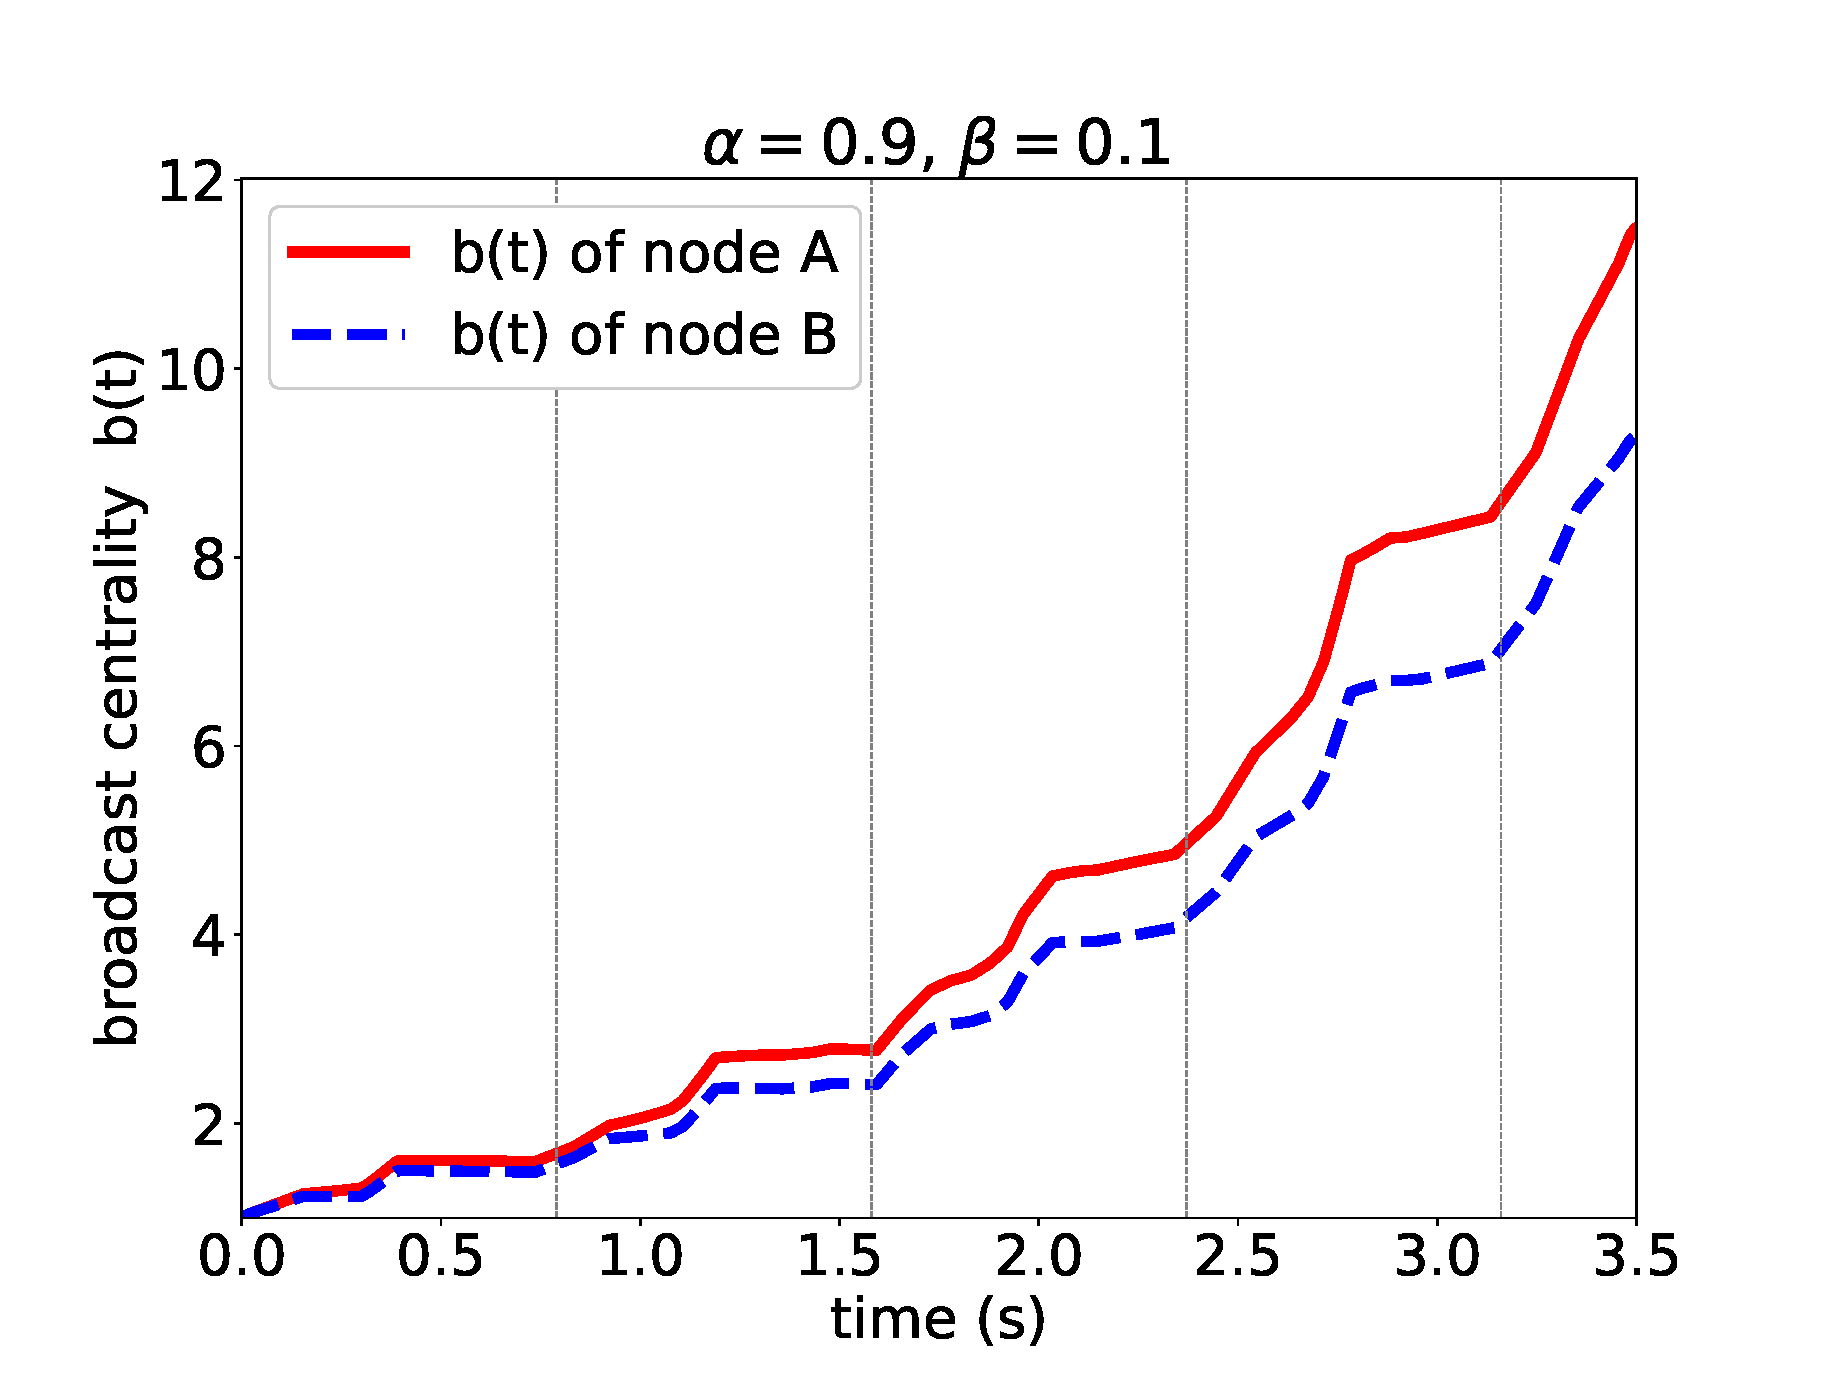
\includegraphics[width=\textwidth]{exp2a_btA_vs_btB}
         \caption{broadcast for $\alpha = 0.9 ,~\beta = 0.1$}
         \label{fig:bt6}
     \end{subfigure}
     \caption{Dynamic broadcast centrality over time for node A (solid) and node B (dashed) in the network of figure \ref{fig:exp2}.}
     \label{fig:twobt}
\end{figure}

\section{Voice call experiment}
\label{sec:voicecall}
The next experiment applies the new modelling framework (Eq. \ref{eqn:u3.3}) to a set of voice call interactions, in order to analyze the dynamic behavior of a fictitious, controversial socio-political movement. The data used for the experiment, supplied as part of the IEEE VAST 2008 Challenge \cite{grinstein2008vast}, consists of a complete set of 9834 time-stamped calls across 400 cell phone users over a 10 day period, with information on IDs for the send and receive nodes, start time in hours/minutes, and duration in seconds.

The aim of the experiment is to show the usefulness of the new matrix ODE in dealing with this type of dynamic network, comparing dynamical measures against aggregated. To that end, the bandwidth of a node is defined as the aggregate number of seconds for which the node ID is active as a sender or receiver. This will allow us to compare the effective activation time of a certain node with its relevance in terms of dynamic broadcast centrality.

The designers of the above mentioned competition provided additional information indicating that node 200 was the leader of an important community who controlled a closely connected subnetwork or inner circle consisting of nodes 1, 2, 3, and 5. However, starting from day 7, these individuals seem to have switched their phone IDs: node 200 became 300, and the others became 306, 309, 360, and 392.

For this experiment, $\mathbf{A}(t)$ was assumed to be symmetric, meaning that $\mathbf{A}_{ij}(t) = \mathbf{A}_{ji}(t) = 1$ if nodes $i$ and $j$ were communicating at time $t$, which was measured in seconds. Parameters $\beta$ was chosen to be approximately $\beta = 1/(60\times 60 \times 24) \approx 1.2 \times 10^{-5}$, which corresponded to a time downweighting of $e^{-1}$ per day, and set the edge attenuation parameter $\alpha$ to a similar value of $10^{-4}$. The SciPy's \texttt{solve\_ivp} method was used to numerically solve the ODE (\ref{eqn:u3.3}), which discretizes the time interval in an efficient and transparent way under the hood. Additionally, absolute and relative error tolerances were both set to $10^{-4}$. To improve efficiency, the matrix logarithm was approximated in this occasion with its expansion to the fifth power:

$$\log(\mathbf{I} - \alpha \mathbf{A}(t)) \approx \alpha \mathbf{A}(t) - \alpha^2 \mathbf{A}(t)^2/2 + \alpha^3 \mathbf{A}(t)^3/3 - \alpha^4 \mathbf{A}(t)^4/4 + \alpha^5 \mathbf{A}(t)^5/5$$ 

Visually speaking, the effects of increasing the number of terms in the expansion to 6 and 7 remained identical.

The experiment yields two key findings:
\begin{enumerate}[label=(\roman*)]
  \item The dynamic broadcast/receive measures (Eqs. \ref{eqn:u3.4}) identified key nodes as highly influential, even if they were not actively using much bandwidth, without any prior knowledge of an inner circle's existence.
  \item The transformation occurred in the network on day 7 was shown by the running centrality measures once we knew the IDs of the inner circle.
\end{enumerate}

\newpage

Figure \ref{fig:ve1a} was used to demonstrate point (i) by plotting bandwidth against dynamic broadcast, $\mathbf{b}(t)$, using data up until the end of day 6. Dynamic receive centrality, $\mathbf{r}(t)$, was also computed using its own vector-valued ODE (Eq. \ref{eqn:u4.1}) obtaining similar results and a computation time reduction of approximately $30\%$. The scatter plot also includes symbols to mark certain nodes, such as a downward pointing triangle for the ring leader, 200, and squares for the related inner-circle nodes, 1, 2, 3, and 5. The follow-on ID for the ringleader, 300, is marked with an upward pointing triangle, and those for other members, 306, 309, 360, and 392, are marked with diamonds.

The results showed that the key nodes for days 1-6 were much more dominant in terms of dynamic broadcast than overall bandwidth. Specifically, the ringleader node had a low bandwidth but ranked sixth out of 400 in terms of broadcast communicability.

\begin{figure}[h]
     \centering
     \begin{subfigure}[b]{0.49\textwidth}
         \centering
         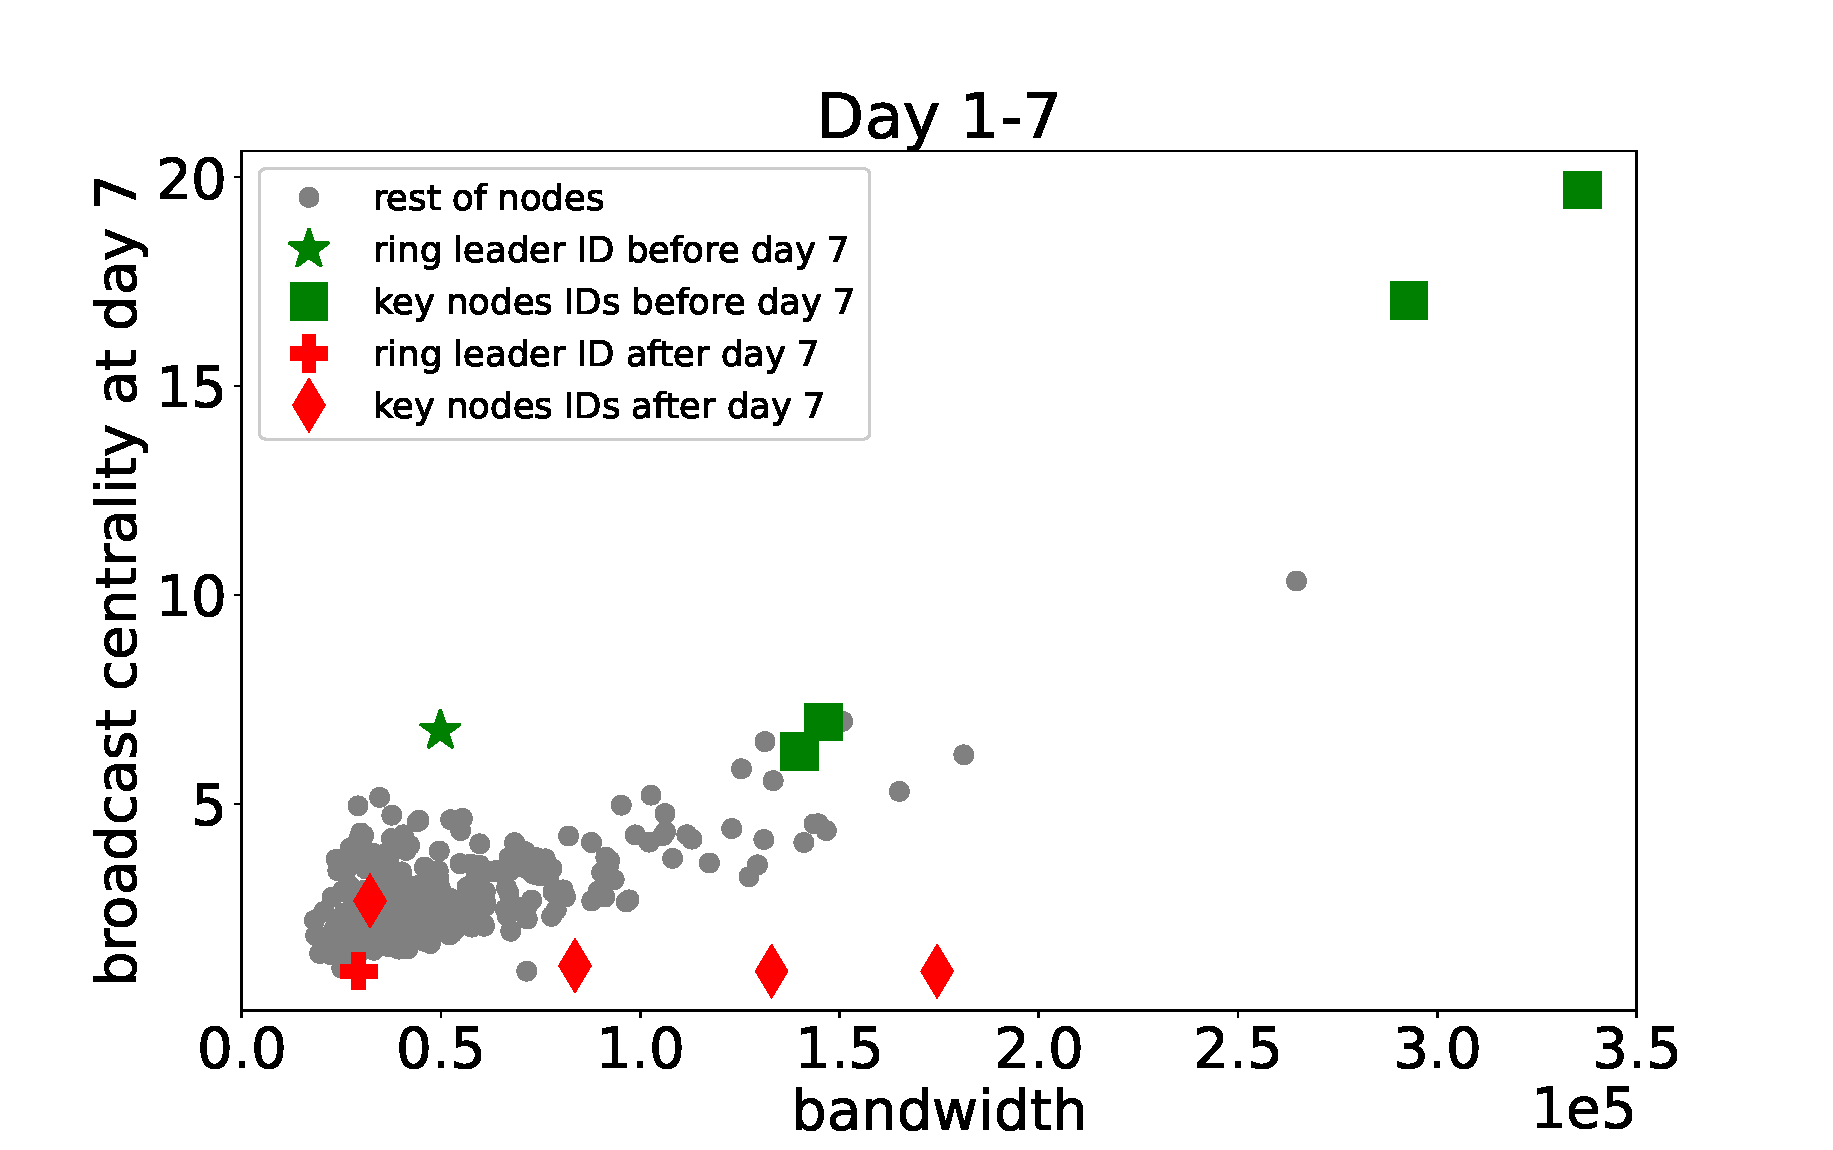
\includegraphics[width=\textwidth]{voicecall_exp_1_7}
         \caption{broadcast centrality at the end of day 6 vs. bandwidth (secs.)}
         \label{fig:ve1a}
     \end{subfigure}
     \hfill
     \begin{subfigure}[b]{0.49\textwidth}
         \centering
         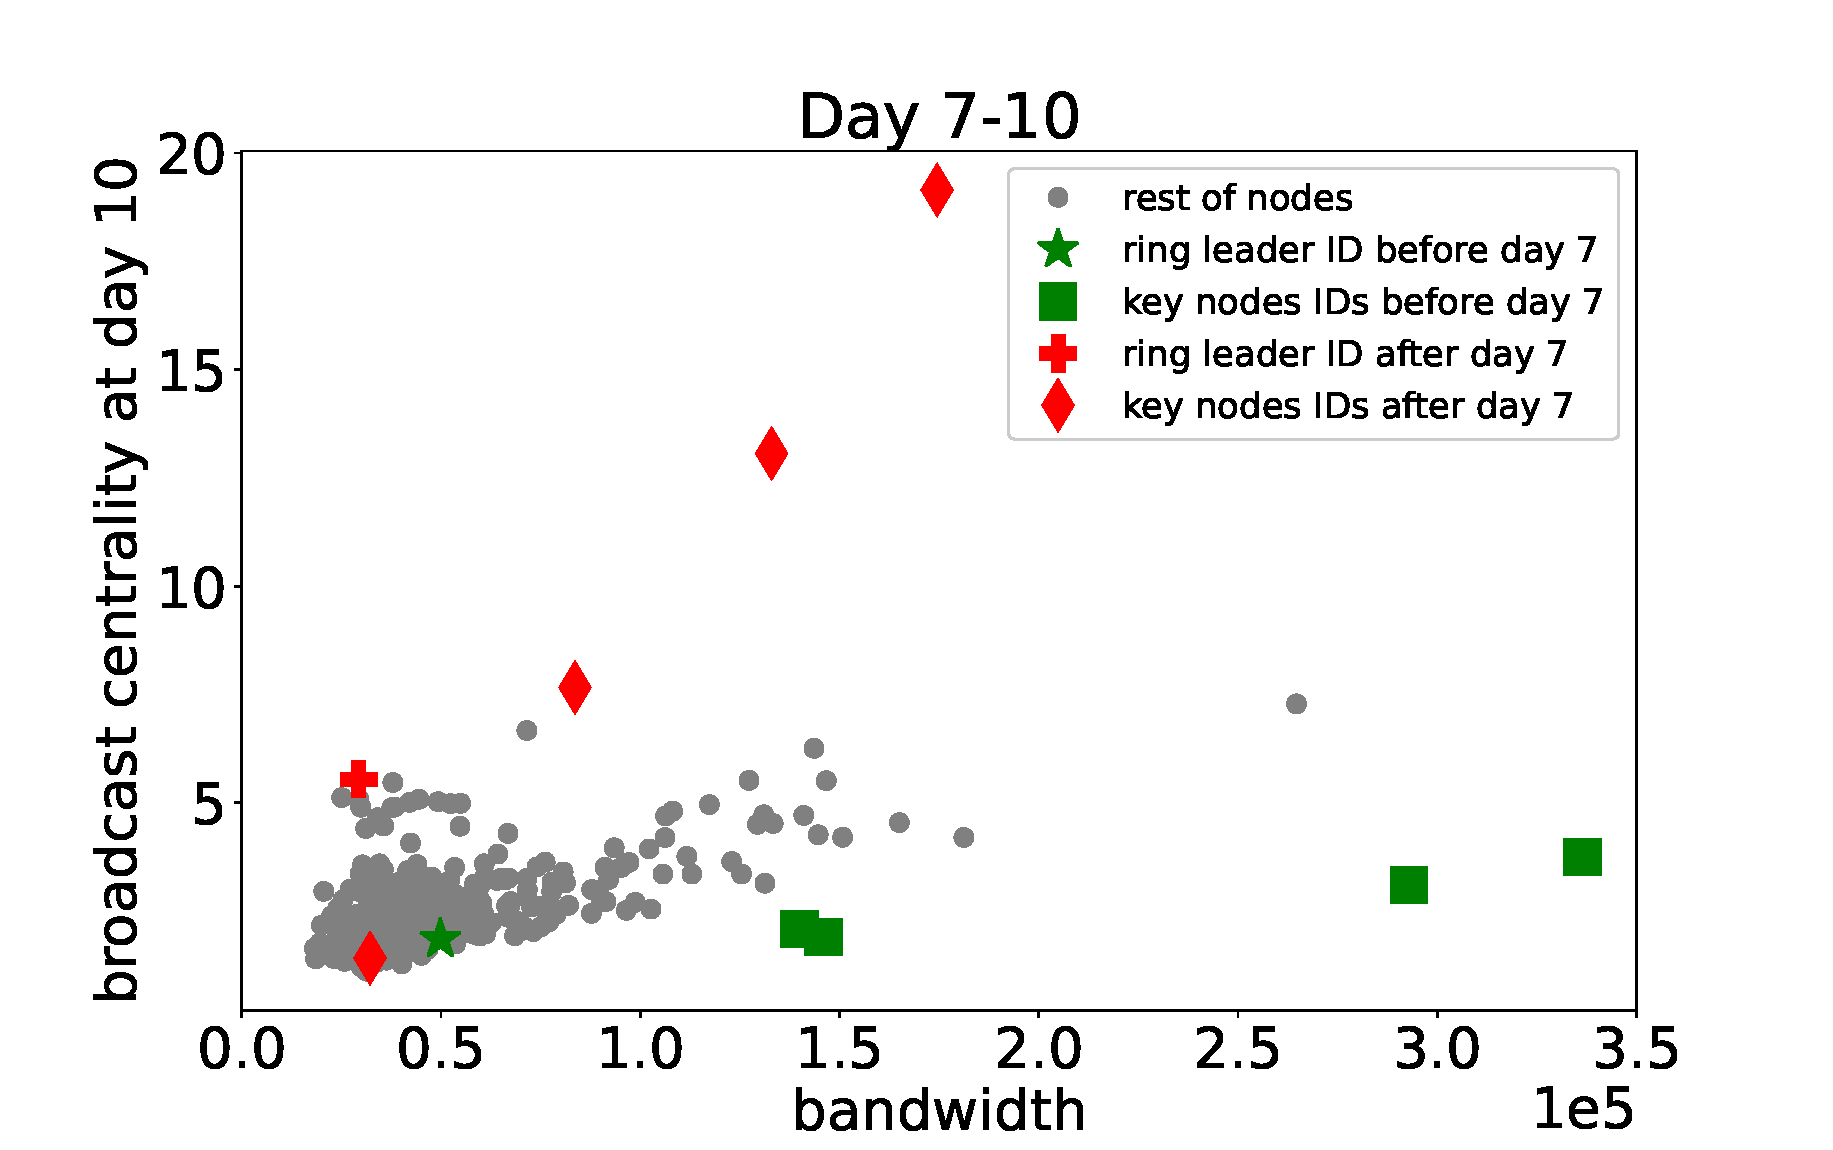
\includegraphics[width=\textwidth]{voicecall_exp_7_10}
         \caption{broadcast centrality at the end of day 10 vs. bandwidth (secs.)}
         \label{fig:ve1b}
     \end{subfigure}
     \caption{Dynamic broadcast measure for each node vs. node's bandwidth from voice call data.}
     \label{fig:ve1}
\end{figure}

The data from days 7 to 10 is displayed in Figure \ref{fig:ve1b}, and it confirms that the dynamic broadcast score is a more effective indicator of centrality than overall bandwidth in uncovering the inner circle. The plot shows how the new ID of the ringleader, that is indicated with an upward pointing triangle, has a low overall bandwidth, but ranks seventh highest for broadcast centrality. Although the former IDs from the inner circle, marked with squares, still possess high bandwidth, their low dynamic broadcast scores suggest that they are no longer central players.

\newpage

The communicability between the original IDs of the five most important players (ID nodes: 200, 1, 2, 3, and 5) is presented in Figure \ref{fig:ve2} to support point (ii). The graph shows how communication between these key nodes changes over a ten days period of time. At each discretized time point, the average amount of messages, broadcast ($U_{ij}$) and received ($U_{ji}$), between each pair of key nodes is measured and then scaled by the average amount of communication between all pairs of nodes in the network. By analyzing this measure, we can observe how the network changes over time, especially when the players start using different IDs after day 7.

\begin{figure}[h]\centering
    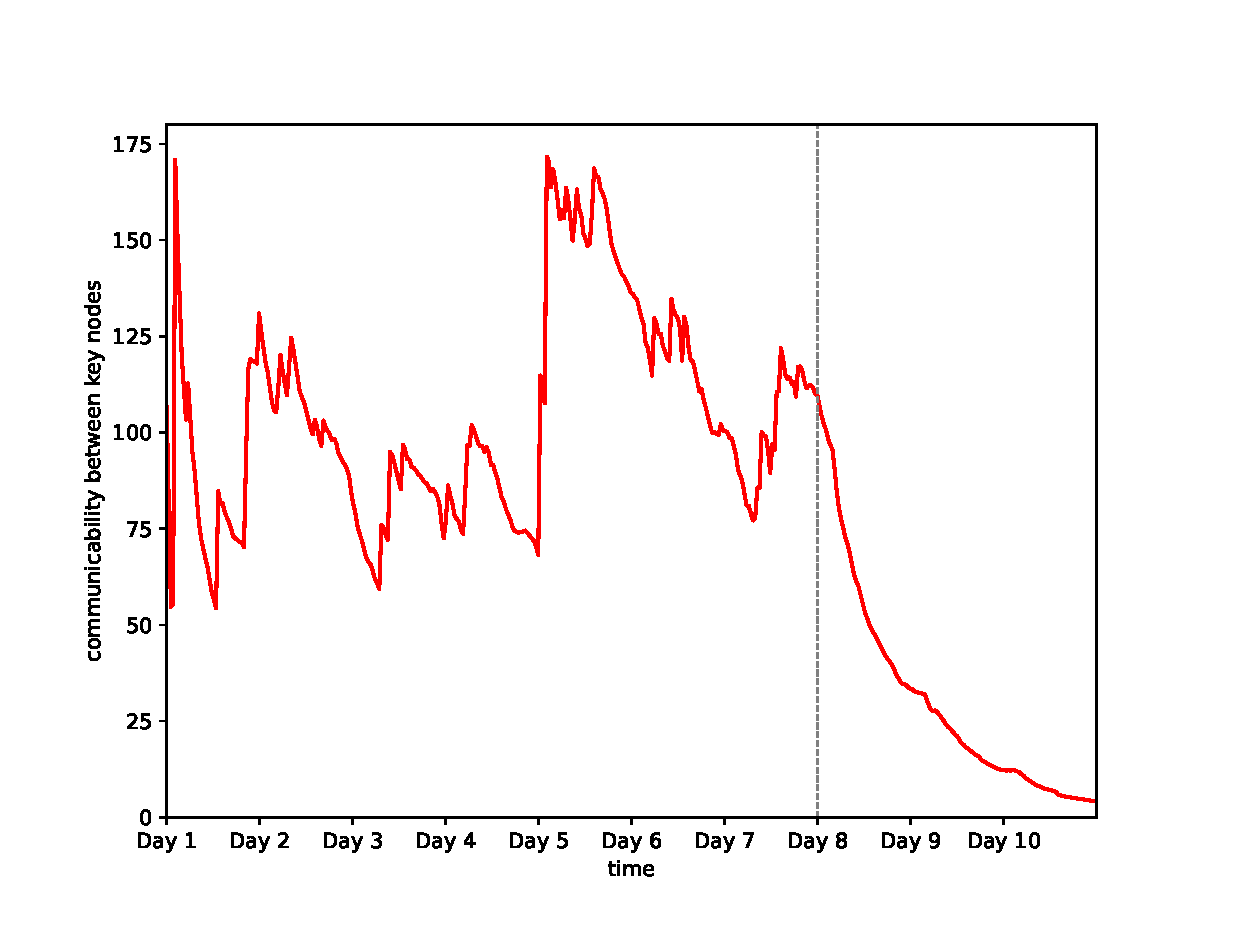
\includegraphics[width=.79\textwidth]{voicecall_exp_dyncomm}
    \caption{Voice call data: dynamic communicability between the five key nodes as a function of time.}
    \label{fig:ve2}
    \bigskip
\end{figure}